%!TEX root = hard_stack_paper/paper.tex


\begin{figure*}[t]

\begin{subfigure}[t]{\textwidth}
\centering
\scalebox{0.6}{
 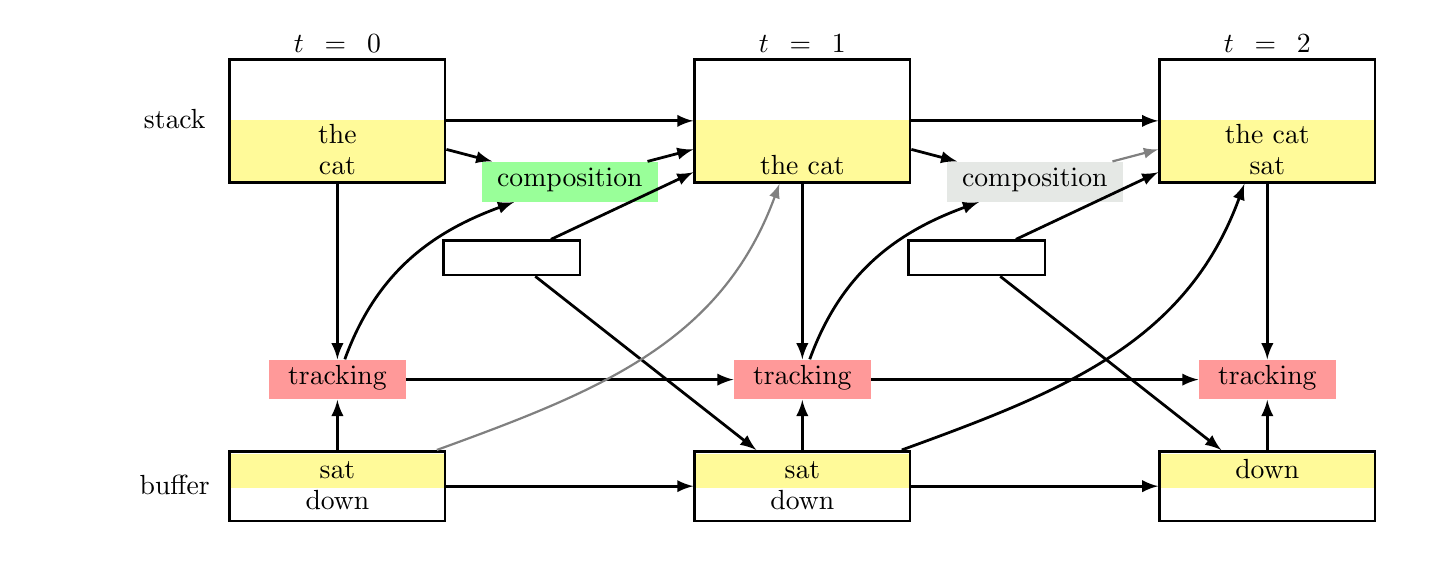
\begin{tikzpicture}
    \def\dx{21pt}
    \def\dy{11pt}
    \def\sy{13*\dy}
    \def\oxb{8*\dx}
    \def\by{1*\dy}
    \def\ox{0*\oxb}

    \tikzstyle{label}=[text width=35mm,align=center,text height=2mm]    
    \tikzstyle{word}=[text width=35mm,align=center,text height=2mm]    
    \tikzstyle{tracker}=[fill=red!40,text width=15mm,align=center,text height=2mm]
    \tikzstyle{softmax}=[fill=blue!40,text width=15mm,align=center,text height=2mm]
    \tikzstyle{comp}=[fill=green!40,text width=20mm,align=center,text height=2mm]
    \tikzstyle{compoff}=[fill=green!10!black!10,text width=20mm,align=center,text height=2mm]
    \tikzstyle{result}=[line width=1pt,draw=black,text width=15mm,align=center,text height=2mm]    
    \tikzstyle{sbox}=[line width=1pt,draw=black,text width=25mm,align=center,text height=13.3mm]
    \tikzstyle{bbox}=[line width=1pt,draw=black,text width=25mm,align=center,text height=6.5mm]
    \tikzstyle{focus1}=[fill=yellow!40,text width=25mm,align=center,text height=2mm]
    \tikzstyle{focus2}=[fill=yellow!40,text width=25mm,align=center,text height=5.5mm]

    \node[label]  (sl) at (\ox-0.35*\oxb+0*\dx,\by+0.5*\dy) {buffer};

    \node[label]  (1l) at (\ox+0*\dx,\sy+3*\dy) {$t=0$};

    \node[focus1] (0bb) at  (\ox+0*\dx,2*\dy) {};
    \node[word]  (0b3) at (\ox+0*\dx,\by-1*\dy) {};
    \node[word]  (0b2) at (\ox+0*\dx,\by+0*\dy) {down};
    \node[word]  (0b1) at (\ox+0*\dx,\by+1*\dy) {sat};
    \node[bbox] (0bb) at  (\ox+0*\dx,\by+0.5*\dy) {};
    
    \node[label]  (sl) at (\ox-0.35*\oxb+0*\dx,\sy+0.5*\dy) {stack};
    
    \node[focus2] (0sb) at  (\ox+0*\dx,\sy-0.5*\dy) {};
    \node[word]  (0s1) at (\ox+0*\dx,\sy-1*\dy) {cat};
    \node[word]  (0s2) at (\ox+0*\dx,\sy+0*\dy) {the};
    \node[word]  (0s3) at (\ox+0*\dx,\sy+1*\dy) {};
    \node[sbox] (0sb) at  (\ox+0*\dx,\sy+0.5*\dy) {};
    
    \node[comp] (0c) at  (\ox+0.5*\oxb,\sy-1.5*\dy) {composition};
    
    \node[tracker] (0t) at  (\ox+0*\dx,5*\dy) {tracking};
    % \node[softmax] (0sm) at  (\ox+3*\dx,7*\dy) {$\sigma$};
    \node[result] (0so) at  (\ox+3*\dx,9*\dy) {\reduce};
    
    \def\ox{1*\oxb}

    \node[label]  (1l) at (\ox+0*\dx,\sy+3*\dy) {$t=1$};

    \node[focus1] (1bb) at  (\ox+0*\dx,2*\dy) {};
    \node[word]  (1b3) at (\ox+0*\dx,\by-1*\dy) {};
    \node[word]  (1b2) at (\ox+0*\dx,\by+0*\dy) {down};
    \node[word]  (1b1) at (\ox+0*\dx,\by+1*\dy) {sat};
    \node[bbox] (1bb) at  (\ox+0*\dx,\by+0.5*\dy) {};
    
    \node[focus2] (1sb) at  (\ox+0*\dx,\sy-0.5*\dy) {};
    \node[word]  (1s1) at (\ox+0*\dx,\sy-1*\dy) {the cat};
    \node[word]  (1s2) at (\ox+0*\dx,\sy+0*\dy) {};
    \node[word]  (1s3) at (\ox+0*\dx,\sy+1*\dy) {};
    \node[sbox] (1sb) at  (\ox+0*\dx,\sy+0.5*\dy) {};
    
    \node[compoff] (1c) at  (\ox+0.5*\oxb,\sy-1.5*\dy) {composition};
    
    \node[tracker] (1t) at  (\ox+0*\dx,5*\dy) {tracking};
    % \node[softmax] (1sm) at  (\ox+3*\dx,7*\dy) {$\sigma$};
    \node[result] (1so) at  (\ox+3*\dx,9*\dy) {\shift};
     
    \def\ox{2*\oxb}

    \node[label]  (1l) at (\ox+0*\dx,\sy+3*\dy) {$t=2$};

    \node[focus1] (2bb) at  (\ox+0*\dx,2*\dy) {};
    \node[word]  (2b3) at (\ox+0*\dx,\by-1*\dy) {};
    \node[word]  (2b2) at (\ox+0*\dx,\by+0*\dy) {};
    \node[word]  (2b1) at (\ox+0*\dx,\by+1*\dy) {down};
    \node[bbox] (2bb) at  (\ox+0*\dx,\by+0.5*\dy) {};
    
    \node[focus2] (2sb) at  (\ox+0*\dx,\sy-0.5*\dy) {};
    \node[word]  (2s1) at (\ox+0*\dx,\sy-1*\dy) {sat};
    \node[word]  (2s2) at (\ox+0*\dx,\sy+0*\dy) {the cat};
    \node[word]  (2s3) at (\ox+0*\dx,\sy+1*\dy) {};
    \node[sbox] (2sb) at  (\ox+0*\dx,\sy+0.5*\dy) {};
   
    \node[tracker] (2t) at  (\ox+0*\dx,5*\dy) {tracking};

    
    \pgfsetarrowsend{latex}
    \tikzstyle{fwd} = [draw=black, line width=1pt]
    \tikzstyle{gated} = [draw=black!50, line width=0.8pt]

    \draw [fwd] (0sb) -- (0t);
    \draw [fwd] (0bb) -- (0t);
    \draw [fwd] (0sb) -- (0c);
    
    \draw [fwd] (0t) -- (1t);
    \draw [fwd] (0t) to[out=70,in=-160] (0c);
    \draw [fwd] (0sb) -- (1sb);
    \draw [fwd] (0bb) -- (1bb);
    \draw [fwd] (0so) -- (1sb);
    \draw [fwd] (0so) -- (1bb);
    \draw [gated] (0bb) to[out=20,in=-110] (1sb);
    \draw [fwd] (0c) -- (1sb);

    \draw [fwd] (1sb) -- (1t);
    \draw [fwd] (1bb) -- (1t);
    \draw [fwd] (1sb) -- (1c);
    
    \draw [fwd] (1t) -- (2t);
    \draw [fwd] (1t) to[out=70,in=-160] (1c);
    \draw [fwd] (1sb) -- (2sb);
    \draw [fwd] (1bb) -- (2bb);
    \draw [fwd] (1so) -- (2sb);
    \draw [fwd] (1so) -- (2bb);
    \draw [fwd] (1bb) to[out=20,in=-110] (2sb);
    \draw [gated] (1c) -- (2sb);

    \draw [fwd] (2sb) -- (2t);
    \draw [fwd] (2bb) -- (2t);


  \end{tikzpicture}}
  
 \caption{The model unrolled for two transitions on the input \word{the cat sat down}.}\label{fig:model:0}
  
\end{subfigure}\\\\\\
\begin{subfigure}[t]{\textwidth}
\centering
\scalebox{0.6}{
 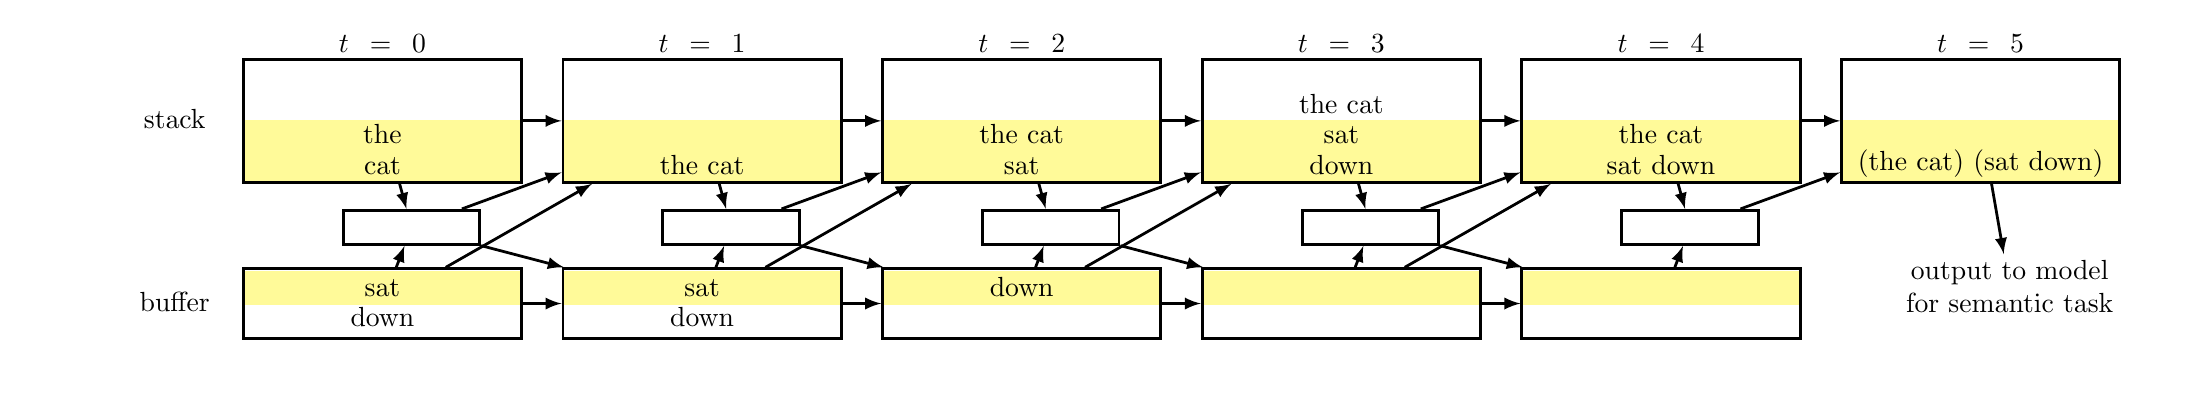
\begin{tikzpicture}
    \def\dx{21pt}
    \def\dy{11pt}
    \def\sy{7*\dy}
    \def\oxb{5.5*\dx}
    \def\by{1*\dy}
    \def\ox{0*\oxb}

    \tikzstyle{label}=[text width=35mm,align=center,text height=2mm]    
    \tikzstyle{word}=[text width=35mm,align=center,text height=2mm]    
    \tikzstyle{tracker}=[fill=red!40,text width=15mm,align=center,text height=2mm]
    \tikzstyle{softmax}=[text width=40mm,align=center,text height=2mm]
    \tikzstyle{comp}=[fill=green!40,text width=20mm,align=center,text height=2mm]
    \tikzstyle{result}=[line width=1pt,draw=black,text width=15mm,align=center,text height=2mm]    
    \tikzstyle{sbox}=[line width=1pt,draw=black,text width=33mm,align=center,text height=13.3mm]
    \tikzstyle{bbox}=[line width=1pt,draw=black,text width=33mm,align=center,text height=6.5mm]
    \tikzstyle{focus1}=[fill=yellow!40,text width=33mm,align=center,text height=2mm]
    \tikzstyle{focus2}=[fill=yellow!40,text width=33mm,align=center,text height=5.5mm]

    \def\ox{0*\oxb}
    
    \node[label]  (1l) at (\ox+0*\dx,\sy+3*\dy) {$t=0$};
    
    \node[label]  (sl) at (\ox-0.65*\oxb+0*\dx,\by+0.5*\dy) {buffer};
    
    \node[focus1] (1bb) at  (\ox+0*\dx,2*\dy) {};
    \node[word]  (1b3) at (\ox+0*\dx,\by-1*\dy) {};
    \node[word]  (1b2) at (\ox+0*\dx,\by+0*\dy) {down};
    \node[word]  (1b1) at (\ox+0*\dx,\by+1*\dy) {sat};
    \node[bbox] (1bb) at  (\ox+0*\dx,\by+0.5*\dy) {};
    
    \node[label]  (sl) at (\ox-0.65*\oxb+0*\dx,\sy+0.5*\dy) {stack};
    
    \node[focus2] (1sb) at  (\ox+0*\dx,\sy-0.5*\dy) {};
    \node[word]  (1s1) at (\ox+0*\dx,\sy-1*\dy) {cat};
    \node[word]  (1s2) at (\ox+0*\dx,\sy+0*\dy) {the};
    \node[word]  (1s3) at (\ox+0*\dx,\sy+1*\dy) {};
    \node[sbox] (1sb) at  (\ox+0*\dx,\sy+0.5*\dy) {};
    
    \node[result] (1so) at  (\ox+0.5*\dx,4*\dy) {\reduce};
              
    \def\ox{1*\oxb}
   
    \node[label]  (1l) at (\ox+0*\dx,\sy+3*\dy) {$t=1$};
    
    \node[focus1] (2bb) at  (\ox+0*\dx,2*\dy) {};
    \node[word]  (2b3) at (\ox+0*\dx,\by-1*\dy) {};
    \node[word]  (2b2) at (\ox+0*\dx,\by+0*\dy) {down};
    \node[word]  (2b1) at (\ox+0*\dx,\by+1*\dy) {sat};
    \node[bbox] (2bb) at  (\ox+0*\dx,\by+0.5*\dy) {};
    
    \node[focus2] (2sb) at  (\ox+0*\dx,\sy-0.5*\dy) {};
    \node[word]  (2s1) at (\ox+0*\dx,\sy-1*\dy) {the cat};
    \node[word]  (2s2) at (\ox+0*\dx,\sy+0*\dy) {};
    \node[word]  (2s3) at (\ox+0*\dx,\sy+1*\dy) {};
    \node[sbox] (2sb) at  (\ox+0*\dx,\sy+0.5*\dy) {};
    
    \node[result] (2so) at  (\ox+0.5*\dx,4*\dy) {\shift};
             
    \def\ox{2*\oxb}
    
    \node[label]  (1l) at (\ox+0*\dx,\sy+3*\dy) {$t=2$};
    
    \node[focus1] (3bb) at  (\ox+0*\dx,2*\dy) {};
    \node[word]  (3b3) at (\ox+0*\dx,\by-1*\dy) {};
    \node[word]  (3b2) at (\ox+0*\dx,\by+0*\dy) {};
    \node[word]  (3b1) at (\ox+0*\dx,\by+1*\dy) {down};
    \node[bbox] (3bb) at  (\ox+0*\dx,\by+0.5*\dy) {};
    
    \node[focus2] (3sb) at  (\ox+0*\dx,\sy-0.5*\dy) {};
    \node[word]  (3s1) at (\ox+0*\dx,\sy-1*\dy) {sat};
    \node[word]  (3s2) at (\ox+0*\dx,\sy+0*\dy) {the cat};
    \node[word]  (3s3) at (\ox+0*\dx,\sy+1*\dy) {};
    \node[sbox] (3sb) at  (\ox+0*\dx,\sy+0.5*\dy) {};
    
    \node[result] (3so) at  (\ox+0.5*\dx,4*\dy) {\shift};

    \def\ox{3*\oxb}
    
    \node[label]  (1l) at (\ox+0*\dx,\sy+3*\dy) {$t=3$};
        
    \node[focus1] (4bb) at  (\ox+0*\dx,2*\dy) {};
    \node[word]  (4b3) at (\ox+0*\dx,\by-1*\dy) {};
    \node[word]  (4b2) at (\ox+0*\dx,\by+0*\dy) {};
    \node[word]  (4b1) at (\ox+0*\dx,\by+1*\dy) {};
    \node[bbox] (4bb) at  (\ox+0*\dx,\by+0.5*\dy) {};
    
    \node[focus2] (4sb) at  (\ox+0*\dx,\sy-0.5*\dy) {};
    \node[word]  (4s1) at (\ox+0*\dx,\sy-1*\dy) {down};
    \node[word]  (4s2) at (\ox+0*\dx,\sy+0*\dy) {sat};
    \node[word]  (4s3) at (\ox+0*\dx,\sy+1*\dy) {the cat};
    \node[sbox] (4sb) at  (\ox+0*\dx,\sy+0.5*\dy) {};
    
    \node[result] (4so) at  (\ox+0.5*\dx,4*\dy) {\reduce};
                  
    \def\ox{4*\oxb}
    
    \node[label]  (1l) at (\ox+0*\dx,\sy+3*\dy) {$t=4$};
    
    \node[focus1] (5bb) at  (\ox+0*\dx,2*\dy) {};
    \node[word]  (5b3) at (\ox+0*\dx,\by-1*\dy) {};
    \node[word]  (5b2) at (\ox+0*\dx,\by+0*\dy) {};
    \node[word]  (5b1) at (\ox+0*\dx,\by+1*\dy) {};
    \node[bbox] (5bb) at  (\ox+0*\dx,\by+0.5*\dy) {};
    
    \node[focus2] (5sb) at  (\ox+0*\dx,\sy-0.5*\dy) {};
    \node[word]  (5s1) at (\ox+0*\dx,\sy-1*\dy) {sat down};
    \node[word]  (5s2) at (\ox+0*\dx,\sy+0*\dy) {the cat};
    \node[word]  (5s3) at (\ox+0*\dx,\sy+1*\dy) {};
    \node[sbox] (5sb) at  (\ox+0*\dx,\sy+0.5*\dy) {};
    
    \node[result] (5so) at  (\ox+0.5*\dx,4*\dy) {\reduce};
    
    \def\ox{5*\oxb}

    \node[label]  (1l) at (\ox+0*\dx,\sy+3*\dy) {$t=5$};

    \node[focus2] (6sb) at  (\ox+0*\dx,\sy-0.5*\dy) {};
    \node[word]  (6s1) at (\ox+0*\dx,\sy-1*\dy) {(the cat) (sat down)};
    \node[word]  (6s2) at (\ox+0*\dx,\sy+0*\dy) {};
    \node[word]  (6s3) at (\ox+0*\dx,\sy+1*\dy) {};
    \node[sbox] (6sb) at  (\ox+0*\dx,\sy+0.5*\dy) {};

    \node[softmax] (6sm) at  (\ox+0.5*\dx,2*\dy) {output to model for semantic task};
                   
    \pgfsetarrowsend{latex}
    \tikzstyle{fwd} = [draw=black, line width=1pt]

   \draw [fwd] (1sb) -- (1so);
   \draw [fwd] (1bb) -- (1so);

    \draw [fwd] (1sb) -- (2sb);
    \draw [fwd] (1bb) -- (2bb);
    \draw [fwd] (1so) -- (2sb);
    \draw [fwd] (1so) -- (2bb);
    \draw [fwd] (1bb) -- (2sb);

   \draw [fwd] (2sb) -- (2so);
   \draw [fwd] (2bb) -- (2so);

    \draw [fwd] (2sb) -- (3sb);
    \draw [fwd] (2bb) -- (3bb);
    \draw [fwd] (2so) -- (3sb);
    \draw [fwd] (2so) -- (3bb);
    \draw [fwd] (2bb) -- (3sb);

   \draw [fwd] (3sb) -- (3so);
   \draw [fwd] (3bb) -- (3so);

    \draw [fwd] (3sb) -- (4sb);
    \draw [fwd] (3bb) -- (4bb);
    \draw [fwd] (3so) -- (4sb);
    \draw [fwd] (3so) -- (4bb);
    \draw [fwd] (3bb) -- (4sb);

   \draw [fwd] (4sb) -- (4so);
   \draw [fwd] (4bb) -- (4so);

    \draw [fwd] (4sb) -- (5sb);
    \draw [fwd] (4bb) -- (5bb);
    \draw [fwd] (4so) -- (5sb);
    \draw [fwd] (4so) -- (5bb);
    \draw [fwd] (4bb) -- (5sb);

   \draw [fwd] (5sb) -- (5so);
   \draw [fwd] (5bb) -- (5so);

    \draw [fwd] (5sb) -- (6sb);
    \draw [fwd] (5so) -- (6sb);

   \draw [fwd] (6sb) -- (6sm);

  \end{tikzpicture}}
  
 \caption{The fully unrolled model for \word{the cat sat down} with some layers omitted for clarity. \todo{[SB] Add in the first two steps.}}\label{fig:model:1b}  
 
\end{subfigure}
\caption{\label{m1-views}Two views of the transition-based sentence model. In both views, the lower boxes represent the input buffer, and the upper boxes represent the stack. Yellow highlighting indicates which portions of these data structures are visible to the tracking LSTM and to the composition function. Thin gray arrows indicate connections which are blocked by a gating function, and so contribute no information. \todo{[SB] Clean up the arrangements of these figures now that we aren't reporting on Models 1/2.}}

\end{figure*}
